%% ═══════════════════════════════════════════════════════════════════════════
%%  Hybrid Semantic Prototype Weighting and Learning-to-Rank
%%  for Automated Bug Assignment
%%  — Short Paper (ACM sigconf format) —
%% ═══════════════════════════════════════════════════════════════════════════
\documentclass[sigconf,review,anonymous]{acmart}

% ── Packages ──────────────────────────────────────────────────────────────────
\usepackage{booktabs}
\usepackage{array}
\usepackage{graphicx}
\usepackage{tikz}

% ── TikZ libraries ────────────────────────────────────────────────────────────
\usetikzlibrary{
  shapes.geometric, shapes.misc,
  arrows.meta, fit,
  positioning, backgrounds,
  calc, shadows.blur
}

% ── Color Palette (restrained academic) ───────────────────────────────────────
\definecolor{navydark}   {HTML}{1B2A4A}
\definecolor{navymid}    {HTML}{2E4A7A}
\definecolor{tealaccent} {HTML}{1A6B72}
\definecolor{slateblue}  {HTML}{3A4F8A}
\definecolor{indigomid}  {HTML}{4A3A8A}
\definecolor{mulberry}   {HTML}{6B2E5A}
\definecolor{crimsonmid} {HTML}{7A2A2A}
\definecolor{forestmid}  {HTML}{1A5C3A}
\definecolor{guardbg}    {HTML}{4A4A4A}
\definecolor{darktext}   {HTML}{1A1A2E}
\definecolor{arrowcol}   {HTML}{5A6A8A}

% ── TikZ Global Styles ────────────────────────────────────────────────────────
\tikzset{
  iobox/.style={
    rectangle, rounded corners=5pt,
    minimum width=7.2cm, minimum height=1.05cm,
    text centered, font=\small\bfseries,
    draw=#1, fill=#1!10, text=#1!80!black, line width=1.2pt
  },
  stepbox/.style={
    rectangle, rounded corners=4pt,
    minimum width=7.2cm, minimum height=1.15cm,
    text centered, font=\small,
    draw=#1, fill=#1!7, text=darktext, line width=0.9pt
  },
  stepnum/.style={
    circle, minimum size=0.58cm,
    fill=#1, text=white,
    font=\bfseries\scriptsize, inner sep=0pt, line width=0pt
  },
  phasegroup/.style={
    rectangle, rounded corners=6pt,
    draw=#1!50, fill=#1!4,
    dashed, line width=0.8pt,
    inner xsep=12pt, inner ysep=8pt
  },
  myarrow/.style={-Stealth, line width=1.2pt, color=arrowcol},
  dasharrow/.style={-Stealth, line width=0.9pt, color=arrowcol, dashed},
  sidenode/.style={
    rectangle, rounded corners=3pt,
    minimum width=3.2cm, minimum height=0.75cm,
    text centered, font=\scriptsize,
    draw=#1!60, fill=#1!6, text=darktext, line width=0.7pt
  },
  guardrail/.style={
    rectangle, rounded corners=4pt,
    dashed, line width=0.8pt,
    minimum width=7.2cm, minimum height=1.0cm,
    text centered, font=\small\itshape,
    draw=guardbg!60, fill=guardbg!6, text=darktext
  }
}

%% ════════════════════════════════════════════════════════════════════════════
%% ACM Metadata
%% ════════════════════════════════════════════════════════════════════════════

\acmConference[ISEC 2027]{20th Innovations in Software Engineering Conference}{Dates TBD, 2027}{Mumbai, India}
\acmBooktitle{Proceedings of the 20th Innovations in Software Engineering Conference (ISEC 2027), Mumbai, India}
\acmPrice{15.00}
\acmISBN{978-1-4503-XXXX-X/27/02}
\acmDOI{10.1145/XXXXXXX.XXXXXXX}

%% CCS Concepts (required by ACM)
\begin{CCSXML}
<ccs2012>
   <concept>
       <concept_id>10011007.10011074.10011099.10011102.10011103</concept_id>
       <concept_desc>Software and its engineering~Software maintenance tools</concept_desc>
       <concept_significance>500</concept_significance>
   </concept>
   <concept>
       <concept_id>10010147.10010257.10010293.10010294</concept_id>
       <concept_desc>Computing methodologies~Learning to rank</concept_desc>
       <concept_significance>500</concept_significance>
   </concept>
   <concept>
       <concept_id>10010147.10010178.10010179</concept_id>
       <concept_desc>Computing methodologies~Natural language processing</concept_desc>
       <concept_significance>300</concept_significance>
   </concept>
</ccs2012>
\end{CCSXML}

\ccsdesc[500]{Software and its engineering~Software maintenance tools}
\ccsdesc[500]{Computing methodologies~Learning to rank}
\ccsdesc[300]{Computing methodologies~Natural language processing}

%% ════════════════════════════════════════════════════════════════════════════
\begin{document}

% ── Title ─────────────────────────────────────────────────────────────────────
\title{Hybrid Semantic Prototype Weighting and Learning-to-Rank for Automated Bug Assignment}

\author{Anonymous Author(s)}
\affiliation{%
  \institution{Omitted for Double-Blind Review}
  \country{}
}

%% ════════════════════════════════════════════════════════════════════════════
%% ABSTRACT
%% ════════════════════════════════════════════════════════════════════════════
\begin{abstract}
Automated bug assignment aims to reduce triage time by recommending suitable
developers to fix newly reported bugs. We propose a pipeline combining
\emph{Hybrid Semantic Prototype Weighting} with a \emph{Learning-to-Rank}
(LTR) model. A Weighted Sum Model first scores candidates using dynamic
weights derived from cosine similarities between the bug embedding and six
curated prototype sentences. An XGBoost Ranker then refines the order using a
19-dimensional feature vector with a confidence-based fallback mechanism.
Evaluated on four open-source Bugzilla repositories (Eclipse IDE, Mozilla
Firefox, Mozilla Core, and Thunderbird), our LTR approach consistently
Firefox, Mozilla Core, and Thunderbird), our LTR approach consistently
outperforms the semantic WSM baseline, achieving Top-1 accuracies ranging
from \textbf{23.00\%} (Eclipse IDE) to \textbf{49.00\%} (Mozilla Core), with up to a \textbf{+13.00pp} improvement over the baseline. By combining static NLP features with dynamic
ranker refinement, our model shows consistent gains across all four projects.
\end{abstract}

\keywords{Bug Assignment, Learning to Rank, Semantic Embeddings, XGBoost, Software Maintenance}

\maketitle

%% ════════════════════════════════════════════════════════════════════════════
%% I. INTRODUCTION
%% ════════════════════════════════════════════════════════════════════════════
\section{Introduction}

Automated bug assignment reduces triage time by recommending developers equipped to fix newly reported bugs. Traditional approaches using TF-IDF or simple classifiers often struggle with vocabulary mismatch and synonyms~\cite{anvik2006triage}. While recent deep learning models and transformers capture rich semantic nuances~\cite{zaidi2022transformers, dipongkor2023transformer}, they often formulate the task as multi-class classification over hundreds of developers. This setup incurs high computational overhead during inference and requires frequent retraining as developer pools change.

To address these limitations, we introduce a hybrid framework bridging modern semantic NLP and Learning-to-Rank (LTR) algorithms. Our approach dynamically scores bug reports against natural language ``prototype sentences'' using static Sentence-BERT (SBERT) embeddings~\cite{reimers2019sentencetransformers}. These semantic features, along with historical developer metrics, are fed into an XGBRanker model~\cite{chen2016xgboost} trained with a pairwise objective~\cite{liu2009ltr}, achieving high precision with low latency and robust fallback mechanisms.

%% ════════════════════════════════════════════════════════════════════════════
%% II. RELATED WORK
%% ════════════════════════════════════════════════════════════════════════════
\section{Related Work}

Early triage systems relied on traditional machine learning with lexical matching, which Xia et al. improved via DevRec~\cite{xia2013devsim} and TopicMiner-MTM~\cite{xia2017topicminer} using developer activity profiles and topic models. Recent state-of-the-art approaches leverage fine-tuned transformers like DeBERTa~\cite{dipongkor2023transformer} to achieve superior classification, albeit at a high computational cost. Alternatively, LTR techniques, such as LambdaMART~\cite{burges2010lambdamart}, optimize the relative ordering of candidates and have been successfully applied to developer ranking~\cite{mkaouer2020ltrdevs}. Our work uniquely combines the efficiency of static SBERT embeddings with the robustness of LambdaMART-powered XGBRanker, bypassing the rigidity of keyword heuristics and the deployment overhead of massive cross-encoders.

%% ════════════════════════════════════════════════════════════════════════════
%% III. METHODOLOGY
%% ════════════════════════════════════════════════════════════════════════════
\section{Methodology}

Figure~\ref{fig:pipeline} illustrates the complete eight-step pipeline from
incoming bug report to final ranked developer list.
The three shaded regions denote the logical phases of the system:
\emph{Encoding}, \emph{Candidate Selection}, and \emph{Ranking}.

\begin{figure*}[t]
\centering
\resizebox{\textwidth}{!}{%
\begin{tikzpicture}[node distance=0.7cm,
                    every node/.style={align=center}]

  \tikzset{
    iobox/.style={
      rectangle, rounded corners=5pt,
      minimum width=10cm, minimum height=1.1cm,
      text centered, font=\normalsize\bfseries,
      draw=#1, fill=#1!10, text=#1!80!black, line width=1.4pt
    },
    stepbox/.style={
      rectangle, rounded corners=4pt,
      minimum width=10cm, minimum height=1.25cm,
      text centered, font=\normalsize,
      draw=#1, fill=#1!7, text=darktext, line width=1.0pt
    },
    guardrail/.style={
      rectangle, rounded corners=4pt, dashed, line width=0.9pt,
      minimum width=10cm, minimum height=1.1cm,
      text centered, font=\normalsize\itshape,
      draw=guardbg!60, fill=guardbg!6, text=darktext
    },
    sidenode/.style={
      rectangle, rounded corners=3pt,
      minimum width=3.8cm, minimum height=0.85cm,
      text centered, font=\small,
      draw=#1!60, fill=#1!8, text=darktext, line width=0.8pt
    },
    stepnum/.style={
      circle, minimum size=0.68cm,
      fill=#1, text=white,
      font=\bfseries\small, inner sep=0pt, line width=0pt
    }
  }

  \node[iobox=navydark] (input) {%
    \textbf{INPUT}\enspace $B_{\text{new}}$: New Bug Report\\[-2pt]
    {\small Historical Bugs $\mathcal{H}$
     \enspace$|$\enspace Prototypes $\mathcal{P}$
     \enspace$|$\enspace XGBRanker $\mathcal{M}$}};

  \node[stepbox=tealaccent, below=0.65cm of input] (s1) {%
    \textbf{Step 1 — Hybrid Feature Extraction}\\[-2pt]
    {\small SentenceTransformer $\;\to\;$ $E_{\text{dense}}^{\text{new}} \in \mathbb{R}^{384}$
     \qquad TF-IDF $\;\to\;$ $E_{\text{sparse}}^{\text{new}}$}};
  \node[stepnum=tealaccent, left=0.25cm of s1.west] {1};

  \node[stepbox=tealaccent, below=0.6cm of s1] (s2) {%
    \textbf{Step 2 — Hybrid Similarity Search}\\[-2pt]
    {\small $S(B_{\text{new}},H_i)
      = 0.5\cdot\cos(E_{\text{dense}})
      + 0.5\cdot\cos(E_{\text{sparse}})$\quad for all $H_i \in \mathcal{H}$}};
  \node[stepnum=tealaccent, left=0.25cm of s2.west] {2};
  \node[sidenode=tealaccent, right=1.4cm of s2.east] (hist)
    {Historical Bugs\\$\mathcal{H}$};
  \draw[dasharrow] (hist.west) -- (s2.east);

  \node[stepbox=slateblue, below=0.6cm of s2] (s34) {%
    \textbf{Steps 3\,\&\,4 — Candidate Extraction \& Hard Filtering}\\[-2pt]
    {\small Top-20 similar bugs $\;\to\;$ candidate pool $C$
     \qquad Remove: on leave \textbf{or} $\mathit{WL} \geq 0.95$}};
  \node[stepnum=slateblue, left=0.25cm of s34.west] {3--4};

  \node[stepbox=indigomid, below=0.6cm of s34] (s56) {%
    \textbf{Steps 5\,\&\,6 — KNN Affinity \& Attribute Matrix}\\[-2pt]
    {\small $A_d = \dfrac{1}{|\mathcal{H}_d|}
             \displaystyle\sum_{h\in\mathcal{H}_d}S(B_{\text{new}},h)$
     \qquad
     $X_d = [\mathit{Exp}_d,\;FT_d,\;SR_d,\;WL_d,\;DS_d,\;A_d]$}};
  \node[stepnum=indigomid, left=0.25cm of s56.west] {5--6};

  \node[stepbox=mulberry, below=0.6cm of s56] (s7) {%
    \textbf{Step 7 — Semantic Prototype Weighting}\\[-2pt]
    {\small Compare $B_{\text{new}}$ vs.\ prototypes $P_j$
     $\;\to\;$ dynamic weight vector
     $W_j \;\propto\; (R_j \cdot M_{\text{sev}}^{(j)}) + 0.05$}};
  \node[stepnum=mulberry, left=0.25cm of s7.west] {7};
  \node[sidenode=mulberry, right=1.4cm of s7.east] (proto)
    {Semantic Prototypes $\mathcal{P}$};
  \draw[dasharrow] (proto.west) -- (s7.east);

  \node[stepbox=crimsonmid, below=0.6cm of s7] (s8a) {%
    \textbf{Step 8a — WSM Baseline Scoring}\\[-2pt]
    {\small $\textit{Score}_{\text{WSM}}(d)
      = \textsc{MinMax}(X_d)\cdot W
        \;\times\; \textit{ExactMatchMultiplier}$}};
  \node[stepnum=crimsonmid, left=0.25cm of s8a.west] {8a};

  \node[stepbox=crimsonmid, below=0.6cm of s8a] (s8b) {%
    \textbf{Step 8b — Learning-to-Rank (XGBRanker)}\\[-2pt]
    {\small 19-dim feature vector $F_d$
     $\;\to\;$
     $\textit{Score}_{\text{LTR}}(d) = \mathcal{M}.\textsc{Predict}(F_d)$}};
  \node[stepnum=crimsonmid, left=0.25cm of s8b.west] {8b};
  \node[sidenode=crimsonmid, right=1.4cm of s8b.east] (model)
    {Pre-trained\\XGBRanker $\mathcal{M}$};
  \draw[dasharrow] (model.west) -- (s8b.east);

  \node[guardrail, below=0.6cm of s8b] (guard) {%
    \textbf{Safety Guardrail:}\enspace
    if $\;\Delta
       = \textit{Score}_{\text{LTR}}[\text{Rank\,1}]
       - \textit{Score}_{\text{LTR}}[\text{Rank\,2}]
       < 0.1$,\enspace
    fall back to sorting by $\textit{Score}_{\text{WSM}}$};

  \node[iobox=forestmid, below=0.65cm of guard] (output) {%
    \textbf{OUTPUT}\enspace $C_{\text{ranked}}$: Ranked Developer List\\[-2pt]
    {\small Top-1 Acc:\;23.00\% (Eclipse)
     \enspace$|$\enspace MRR:\;0.3254}};

  \foreach \a/\b in {input/s1, s1/s2, s2/s34, s34/s56,
                     s56/s7, s7/s8a, s8a/s8b, s8b/guard, guard/output}{
    \draw[myarrow] (\a) -- (\b);
  }

  \begin{scope}[on background layer]
    \node[phasegroup=tealaccent, fit=(s1)(s2),
          label={[font=\small\bfseries, text=tealaccent!80, xshift=8pt]above left:Encoding Phase}] {};
    \node[phasegroup=slateblue, fit=(s34)(s56),
          label={[font=\small\bfseries, text=slateblue!80, xshift=8pt]above left:Candidate Phase}] {};
    \node[phasegroup=crimsonmid, fit=(s7)(s8a)(s8b),
          label={[font=\small\bfseries, text=crimsonmid!80, xshift=8pt]above left:Ranking Phase}] {};
  \end{scope}

\end{tikzpicture}%
}
\caption{End-to-end automated bug assignment pipeline. Solid arrows denote
         the main data flow; dashed arrows indicate auxiliary data-source
         injections. Shaded regions mark the three logical phases.}
\label{fig:pipeline}
\end{figure*}

Our methodology operates through a progressive pipeline (Figure~\ref{fig:pipeline}) that narrows down an open pool of developers to a confidently ranked list. The process begins with hybrid feature extraction, generating both a dense semantic embedding ($E_{\text{dense}}$) via Sentence-BERT and a sparse lexical embedding ($E_{\text{sparse}}$) via TF-IDF. We compute a hybrid similarity score by averaging the cosine similarities of both representations against historical bugs. We extract the top 20 most similar historical bugs and compile a preliminary candidate pool of developers who successfully resolved them, applying a hard filter to remove developers on leave or with workload $\geq 95\%$.

Next, we calculate a topical expertise score, called KNN Affinity ($A_d$), which averages the hybrid similarities of historical bugs fixed by that specific developer. We then construct a six-dimensional attribute matrix for each candidate: Experience, Fix Time, Success Rate, Workload, Domain Skill, and KNN Affinity.

To dynamically weight these attributes, we use Semantic Prototype Weighting. We define six natural language ``prototype sentences'' representing ideal scenarios (e.g., ``Resolving this bug requires deep expertise''). We compute a prototype score via cosine similarity between the new bug and each prototype sentence, scaled by a severity multiplier. This yields a dynamic weight vector $W$.

In the final ranking phase, a Weighted Sum Model (WSM) baseline computes an initial score via the dot product of the normalized attribute matrix and $W$. We then extract a comprehensive 19-dimensional feature vector (core attributes, interactions, severity, and prototype scores) for each candidate. An XGBRanker model uses these features to generate the primary ranking score. If the ranker's confidence gap between the top two candidates is less than $0.1$, the system safely reverts to the WSM baseline score.

%% ════════════════════════════════════════════════════════════════════════════
%% IV. EXPERIMENTAL SETUP
%% ════════════════════════════════════════════════════════════════════════════
\section{Experimental Setup}

We evaluate on bug report repositories from four large-scale open-source projects hosted on Bugzilla (Table~\ref{tab:projects}). To prevent data leakage, all datasets were strictly evaluated using a chronological split, reserving the most recent 200 bug reports as the test set and utilizing the remaining historical bugs for training (Eclipse IDE: 9,800 train; Mozilla Firefox: 15,192 train; Mozilla Core: 85,352 train; Thunderbird: 5,029 train). For our baseline evaluation, we detail the metrics on the Eclipse IDE dataset~\cite{lamkanfi2013msr}.

\begin{table}[t]
\centering
\small
\caption{Target projects and their repository characteristics.}
\label{tab:projects}
\renewcommand{\arraystretch}{1.2}
\begin{tabular}{@{}lrrr@{}}
\toprule
\textbf{Project} & \textbf{Bugs} & \textbf{Devs} & \textbf{Comps} \\
\midrule
Eclipse IDE     & 10,000 & 209   & 23  \\
Mozilla Firefox & 15,392 & 854   & 50  \\
Mozilla Core    & 85,552 & 2,033 & 179 \\
Thunderbird     & 5,229  & 341   & 22  \\
\bottomrule
\end{tabular}
\end{table}

We report \textbf{Top-$N$ Accuracy} --- the percentage of test bugs for which
the actual resolver appeared in the Top~$N$ recommendations --- for
$N \in \{1, 3, 5\}$, and the \textbf{Mean Reciprocal Rank} (MRR):

\begin{equation}
\text{MRR} = \frac{1}{|Q|}\sum_{i=1}^{|Q|}\frac{1}{\text{rank}_i}
\label{eq:mrr}
\end{equation}

%% ════════════════════════════════════════════════════════════════════════════
%% V. RESULTS & DISCUSSION
%% ════════════════════════════════════════════════════════════════════════════
\section{Results and Discussion}

To evaluate the generalization of our Hybrid Semantic Prototype Weighting and XGBRanker framework, we present a comparative evaluation across the four repositories in Table~\ref{tab:multi_project_results}.

\begin{table*}[t]
\centering
\caption{Performance Comparison of WSM Baseline and XGBRanker (LTR) Across Open-Source Repositories}
\label{tab:multi_project_results}
\renewcommand{\arraystretch}{1.2}
\begin{tabular}{lcccccccc}
\toprule
 & \multicolumn{2}{c}{\textbf{Top-1 Acc.\ (\%)}} & \multicolumn{2}{c}{\textbf{Top-3 Acc.\ (\%)}} & \multicolumn{2}{c}{\textbf{Top-5 Acc.\ (\%)}} & \multicolumn{2}{c}{\textbf{MRR}} \\
\cmidrule(lr){2-3} \cmidrule(lr){4-5} \cmidrule(lr){6-7} \cmidrule(lr){8-9}
\textbf{Project} & \textbf{WSM} & \textbf{LTR} & \textbf{WSM} & \textbf{LTR} & \textbf{WSM} & \textbf{LTR} & \textbf{WSM} & \textbf{LTR} \\
\midrule
Eclipse IDE & 10.00 & \textbf{23.00} & 30.50 & \textbf{41.00} & 38.50 & \textbf{44.50} & 0.2198 & \textbf{0.3254} \\
Mozilla Firefox & 26.50 & \textbf{34.00} & 52.50 & \textbf{58.50} & 61.50 & \textbf{65.50} & 0.4076 & \textbf{0.4721} \\
Mozilla Core & 44.00 & \textbf{49.00} & 64.00 & \textbf{70.00} & 72.50 & \textbf{72.50} & 0.5540 & \textbf{0.5954} \\
Thunderbird & 27.00 & \textbf{34.50} & 57.50 & \textbf{60.50} & 64.50 & \textbf{66.50} & 0.4309 & \textbf{0.4744} \\
\bottomrule
\end{tabular}
\end{table*}

The XGBRanker (LTR) consistently outperforms the WSM baseline across all repositories, achieving absolute Top-1 improvements ranging from +5.0\% (Mozilla Core) to an impressive +13.0\% (Eclipse IDE). Notably, the strict chronological evaluation exposes a severe degradation in the WSM baseline on Eclipse (dropping to 10.00\% Top-1). Standard random cross-validation often artificially inflates baseline metrics by leaking future developer activity into the training context. By contrast, the LTR model's robust 23.00\% Top-1 accuracy demonstrates that its dense semantic features and developer workload heuristics generalize far better to strict temporal boundaries, where the model must assign bugs without knowledge of future repository states. While the LTR increases inference latency slightly (from 58.0\,ms to 150.0\,ms per bug for Eclipse), it remains highly efficient for real-world triaging compared to fine-tuned transformer cross-encoders.

Absolute accuracy varies across projects due to three structural factors: candidate pool size, historical training density, and component granularity. For example, Mozilla Core's massive historical context and high bugs-per-developer average yield the highest absolute Top-1 accuracy (49.00\%). Conversely, Eclipse IDE's challenging assignment environment restricts baseline Top-1 accuracy to 10.00\%, yet the LTR model still achieves 23.00\% Top-1 accuracy, representing the largest relative gain. Despite structural challenges across different organizations, the LTR model's relative improvement remains remarkably consistent, demonstrating robust feature generalization.

%% ════════════════════════════════════════════════════════════════════════════
%% VI. CONCLUSION
%% ════════════════════════════════════════════════════════════════════════════
\section{Conclusion}

We presented a modern architecture for automated bug assignment, combining static dense semantic embeddings with pairwise learning-to-rank to replace rigid keyword heuristics. Evaluated across four major open-source projects, our Hybrid Semantic LTR pipeline demonstrated consistent Top-1 accuracy improvements over WSM baselines while maintaining sub-200\,ms inference latencies. Our analysis highlights that candidate pool size and developer concentration critically govern assignment difficulty.

Future work will explore continuous online learning to update ranker models dynamically.

%% ── References ───────────────────────────────────────────────────────────────
\bibliographystyle{ACM-Reference-Format}
\bibliography{references}

\end{document}
